%\VignetteIndexEntry{Getting started with the package}
%\VignetteKeywords{getting started}
%\VignettePackage{synbreed}

\documentclass[a4paper,11pt]{article}
\usepackage{natbib}
\bibliographystyle{apalike}

% Preabmle parts
\usepackage[T1]{fontenc}
\usepackage{url}
\usepackage{hyperref}
\usepackage{times}

%PSTricks
\usepackage{pdftricks}
\begin{psinputs}
  \usepackage{pst-all}
\end{psinputs}

\usepackage{bm}
\usepackage{amsmath}
\usepackage{amssymb}
\usepackage{latexsym}
\usepackage{verbatim}
\usepackage{epsfig}
\usepackage{comment}
\usepackage{pdfpages}
\usepackage{algorithm2e}

\usepackage{Sweave}
\usepackage{fancyvrb}
\definecolor{Sinput}{rgb}{0.56,0,0}
\DefineVerbatimEnvironment{Sinput}{Verbatim}{formatcom={\color{Sinput}},fontsize=\small,fontshape=sl}
\definecolor{Soutput}{rgb}{0,0,0.56}
\DefineVerbatimEnvironment{Soutput}{Verbatim}{formatcom={\color{Soutput}},fontsize=\small,fontshape=sl}


\title{The R-Package 'synbreed'}
\author{
Valentin Wimmer\thanks{Author of correspondance. Contact: Institute for plant breeding, Technical University of Munich, Emil-Ramann-Str. 4,
	85354 Freising, Germany, Email: \texttt{Valentin.Wimmer@wzw.tum.de}}\\
} \date{\today}

\begin{document}
%%%%%%%%%%%%%%%%%%%%%%%%%%%%%%%%%%%%%%%%%%%%%%%%%%%%%%%%%%%%%%%%%%%%%%
% Sweave
%%%%%%%%%%%%%%%%%%%%%%%%%%%%%%%%%%%%%%%%%%%%%%%%%%%%%%%%%%%%%%%%%%%%%%
%Put all in another directory

 \setkeys{Gin}{width=0.9\textwidth}

%%%%%%%%%%%%%%%%%%%%%%%%%%%%%%%%%%%%%%%%%%%%%%%%%%%%%%%%%%%%%%%%%%%%%%
% Initial R code
%%%%%%%%%%%%%%%%%%%%%%%%%%%%%%%%%%%%%%%%%%%%%%%%%%%%%%%%%%%%%%%%%%%%%%




\maketitle


\begin{abstract}
  \noindent This document gives an introduction to the R-package
  'synbreed' which contains tools and methods for plant and animal breeding. The goal is the creation of an analysis pipeline for genomic selection. This comprises tools
  for genotypic, phenotypic and pedigree data. The steps of a typical analysis are presented in this document. This starts with the coding of the marker data, followed by the construction of relationship matrices according
  to pedigree or genomic relationship matrices based on marker data, i.e. according to \citet{vanRaden2008}. At the end the use of linear mixed models for genomic selection are descriped. \\

  \noindent{\bf Keywords:} synergistic plant and animal breeding, kinship, pedigree, genomic marker data, mixed models, genomic selection
  

  
\end{abstract}


\section{Introduction}\label{sec:Introduction}

The R-package 'synbreed' aims to provide the tools that are necassary to analyze data of breeding programs and perform genomic selecton. Of course, allready
a huge number of software exists for this purpose. The idea of this package is to collect the methods in one package, so that analysis can be performed in one software with just a few steps as descriped in this document. 
Additional, this package takes care of special problems of modern breeding programms as the use of doupled haploid (DH) lines in plant breeding.  Most of packages source code is written in R, so that methods could 
easily be adopted for special purposes.

In this document, the term \textit{genotype} refers to an individuals set of genomic attributes and thus is synonym for an individual. The \textit{phenotype} denotes the observed value of an genotype, i.e. a trait
of commercial interst in breeding programms. The term \textit{genomic markers} refers to a \textit{locus} on the genome where the individuals alleles are measured. At the moment,
the package deals only with two different alleles for each locus which hold if biallelic SNP (single nucleotid polymorphism) markers are used.

The idea of \textit{genomic selection} is that some of the markers are linked to a \textit{quantitative trait loci} (QTL) with an effect on a quantitative phenotypic values. \citet{Meuwissen2001} proposed to make
use of the markers an regress the phenotype on the genotype. The esimated could be used to select the genotypes which a favourable set of genes and select the for the next breeding scheme.

The remainder of the document is structured as follows. In section \ref{sec:ExampleData} a simulated data set is presented which is used to illustrate the methods throughout the document. Section \ref{sec:MarkerData} describes the formatting of marker data  and section \ref{sec:Pedigree} shows how to utilize pedigree information.
In section \ref{sec:RelationshipMatrices} several methods to set up relationship matrices are presented.




\section{Example data}\label{sec:ExampleData}

In this document the steps of an analysis pipline for genotypic and phenotypic data in plant or animal breeding with the R-package 'synbreed' are presented. For illustration, a simulated data set for maize called \texttt{maize}, which is part of the package, is used. 
To load \texttt{maize} data, use
\begin{Schunk}
\begin{Sinput}
> library(synbreed)
> data(maize)
\end{Sinput}
\end{Schunk}
This data set contains genotypic and phenotypic data, as well as pedigree information up to grand parents for 1250 maize lines. When loading \texttt{maize} data, in fact the following
four data sets are loaded into workspace
\begin{description}
\item[maize.geno]  This is a \texttt{data.frame} containing the marker data of 696 biallelic SNP-markers for the 1250 genotypes. 
The first column of the data set contains the \texttt{ID} for the identification of the genotypes.
This variable should be used for the merge with the phenotypic data. 
The marker data is coded with 0/1 and because of simulated data no missing values are present. 
Note that the coding does not contain any information about allel frequencies, thus 1 could be minor or major allele.
\item[maize.pheno] This is a \texttt{data.frame} has one column \texttt{ID} and a column \texttt{Trait} containing the measured phenotypic trait. The order of the genotypes is the same as the order of rows in \texttt{maize.geno}.
\item[maize.ped] This  \texttt{data.frame} contains the pedigree information of  1301 genotypes (1250 lines and 51 ancestors). 
\item[maize.marker.pos]  This  \texttt{data.frame} contains additional information for the SNP markers. The first column \texttt{pos} gives the position of the marker on the chromosome in cM. The second column \texttt{chr} sepecifies the chromosome (linkage group) the marker belongs to. The order of the markers is the same as the order of columns in \texttt{maize.geno}.
\end{description}

\section{Marker data}\label{sec:Markerdata}

In the first step, marker data has to be coded in a way that it could be used for the construction of genomic relationship matrices. For biallelic marker data, the minor allele should be coded as 2 and the major allele as 0.
This task is done by the function \texttt{codeGeno}. If no missing values and heterozygous genotypes are present 
and all markers should be used in the following analyses, this function does simply recode the alleles as mentioned above.
For the \texttt{maize} data, use
\begin{Schunk}
\begin{Sinput}
> marker <- codeGeno(maize.geno[, -1])
\end{Sinput}
\end{Schunk}
to obtain a object \texttt{marker} which contains the recoded marker data. 
Note that the first column is not used because it contains the \texttt{ID}. 
Now, the minor allele frequencies are easily obtained by dividing the column means of \texttt{marker} by 2. 
A histogramm of the minor allele frequencies is shown in Figure \ref{fig:histmaf}.

\begin{figure}[h]
\centering
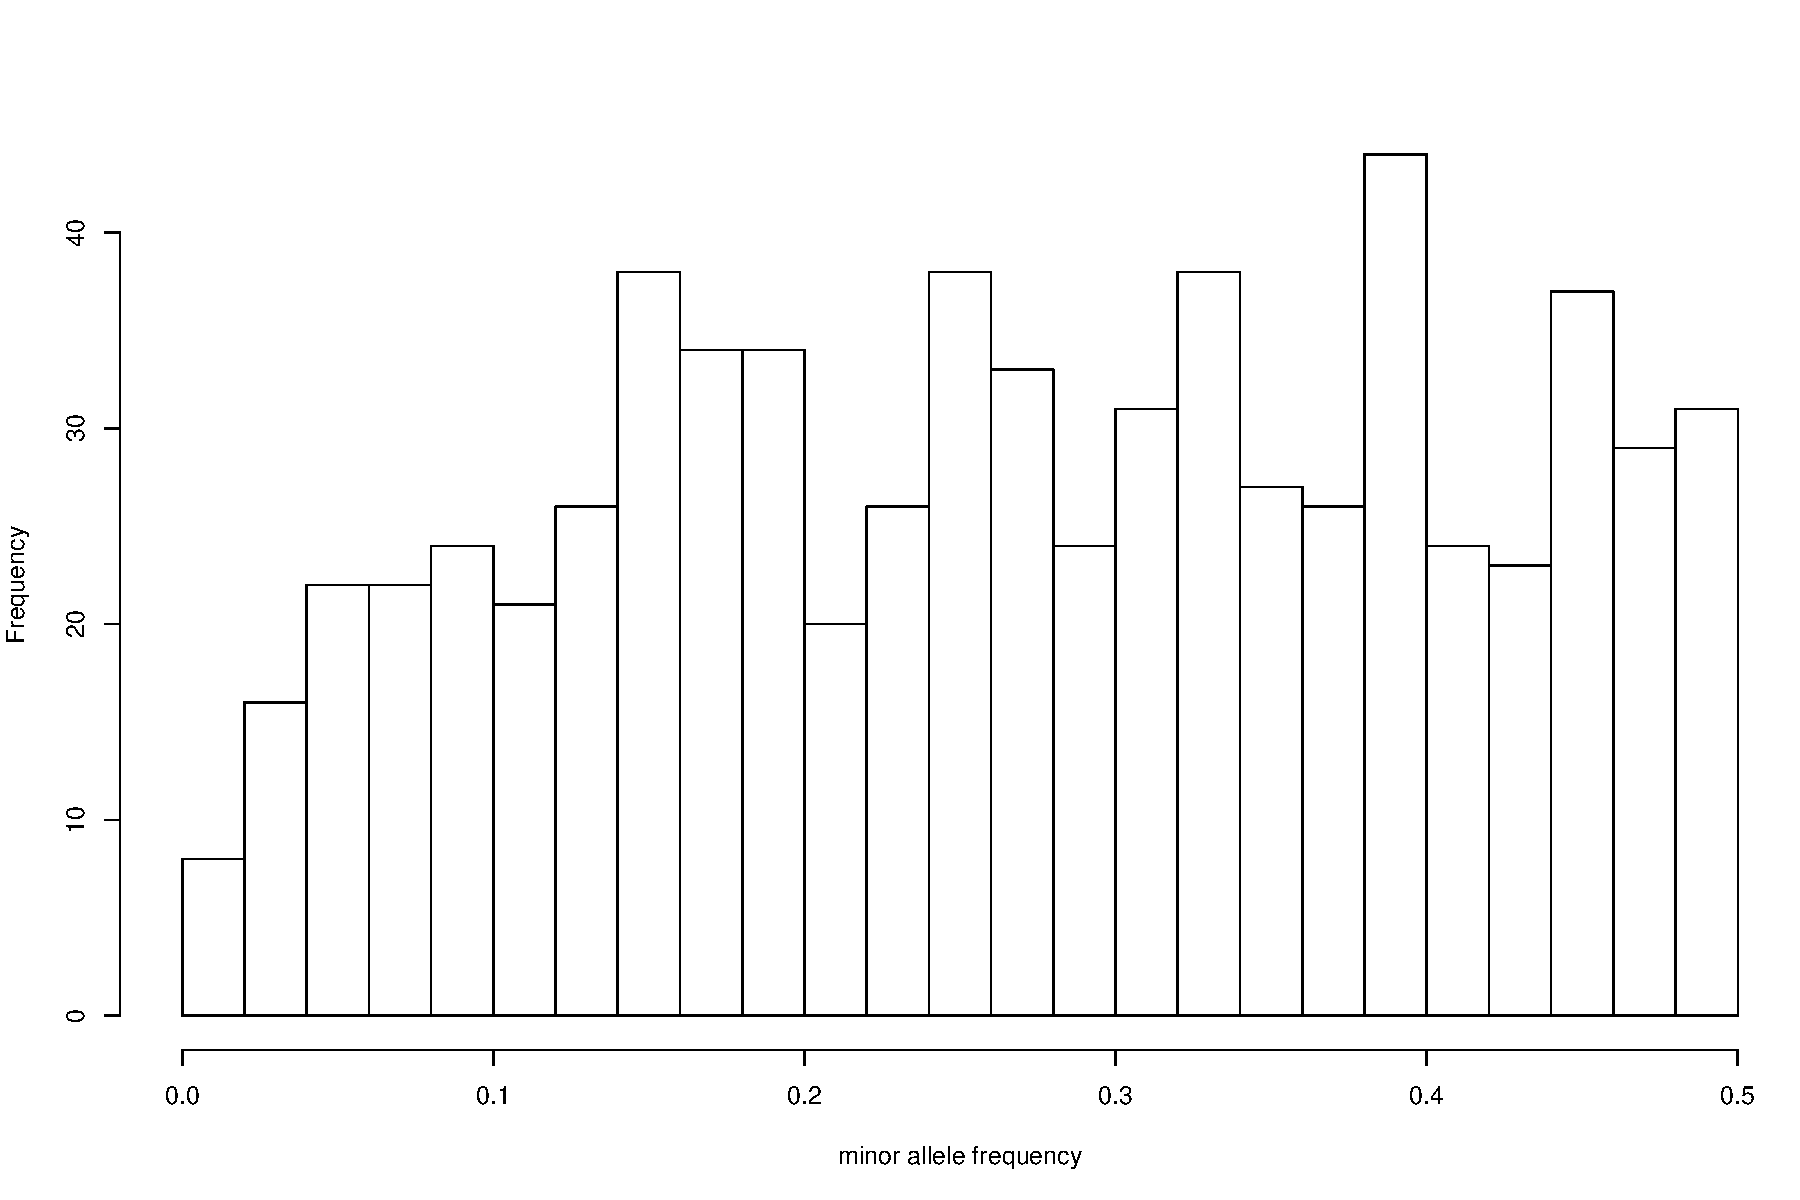
\includegraphics{figs/vignette-004}
\caption{Histogramm of the minor allele frequency of the 696 SNP markers in \texttt{maize} data.}
\label{fig:histmaf}
\end{figure}

In experimental data usually missing values occour in genotypic data due to different reasons 
(i.e. heterozygous genotypes for one locus in homozygous lines).  
The function \texttt{codeGeno} provides the possibility to impute missing values by chance or according to family structure using the following rules:
\begin{description}
\item[with population structure]
Suppose an observation $i$ is missing (NA) for a marker $j$ in population $k$. If marker $j$ is fixed in population $k$, 
the imputed value will be the fixed allele. If marker $j$ is segregating in population $k$, 
the value is 0 with probability 0.5 and 2 with probability 0.5.
\item[without population structure] The missing values for a marker $j$ are sampled from the allele distribution of marker $j$.
\end{description}           
To illustrate the difference in classification of missing values, 200 entries of the marker matrix are selected, the values saved and these entries are coded as \texttt{NA}. 
\begin{Schunk}
\begin{Sinput}
> marker <- as.matrix(marker)
> ind1 <- sample(1:nrow(marker), 200)
> ind2 <- sample(1:ncol(marker), 200)
> posNA <- cbind(ind1, ind2)
> original <- marker[posNA]
> marker[posNA] <- NA
\end{Sinput}
\end{Schunk}
The number of  1250 genotypes in the \texttt{maize} data consist of 25 \textit{half sib} families with 50 genotypes in each family. The genotypes are ordered according to the family structure. 
\begin{Schunk}
\begin{Sinput}
> pop <- rep(1:25, each = 50)
\end{Sinput}
\end{Schunk}
Recoding of the marker data and imputing of the missing  values is done as follows
\begin{Schunk}
\begin{Sinput}
> marker1 <- codeGeno(marker, impute = TRUE, pop)
\end{Sinput}
\begin{Soutput}
approximative run time  6.96  seconds 
 ... 
Total number of missing values                : 200 
Number of imputations by family structure     : 123 
Number of random imputations                  : 77 
Approximative fraction of correct imputations : 0.808 
\end{Soutput}
\end{Schunk}
A report is printed on the screen which informs about the number of imputations performed according to family structure $n_F$ or chance $n_R$. The approximative fraction of correct imputations is $\frac{n_F + 0.5n_R}{n_F+n_R}$. For the simulated data the 
original values are known. With the following commands the quality of the classification of the missing values is judged: 
\begin{Schunk}
\begin{Sinput}
> imputed <- marker1[posNA]
> (t1 <- table(original, imputed))
\end{Sinput}
\begin{Soutput}
        imputed
original   0   2
       0 128  18
       2  24  30
\end{Soutput}
\end{Schunk}
The fraction of correct replacements is
\begin{Schunk}
\begin{Sinput}
> sum(diag(t1))/sum(t1)
\end{Sinput}
\begin{Soutput}
[1] 0.79
\end{Soutput}
\end{Schunk}
Note that expected fraction of correct imputation without family structure equals 0.5.

In an analysis of genotypic data it is common to discard marker with a small minor allele frequency and/or many missing values. 
There are two additional arguments \texttt{maf} and \texttt{nmiss} for function \texttt{codeGeno}. 
Before recoding the data all marker with more than
\texttt{nmiss}$\cdot 100\%$ missing values are discarded. 
After recoding the maker data only markers with a minor allele frequency $>$ \texttt{maf} are returned by the function. 
By default, no markers are selected by one of both criteria, thus \texttt{maf}=\texttt{nmiss}=0.
                                       
%To summarize, the steps presented in Algorithm \ref{alg:codeGeno} are performed.

%\begin{algorithm}[H]
%\SetAlgoLined
%\KwData{\texttt{data.frame} or \texttt{matrix} with $M$ biallelic marker data coded arbitrarily and missing data for $n$ genotypes $g_{ij}$.}
%\KwResult{Marker data without missing vaules with minor allele coded as 2 and major allele coded as 0.}
%\For{$j=$1 to $M$ }{
%\lIf{\% missings $>$ nmiss$\cdot 100\%$} discard marker $j$\;
%\lElse{}{
%Create frequency table for allele $A_1$ and $A_2$ for marker $j$\;
%Order alleles decreasingby their frequencies $f(A_{(1)}) > f(A_{(2)})$\;
%}
%\For{$i=1$ to $n$}{
%\lIf{$g_{ij}$ = $A_{(1)}$}{
%$g_{ij}$ = 0\;
%}
%\lIf{$g_{ij}$ = $A_{(2)}$}{
%$g_{ij}$ = 2\;
%}
%\lElse{}{
%\lIf{$\bs{g}_i$ is segregating in family of genotype $i$}{
%$g_{ij} = \left\{ \begin{array}{ll} 0 & p=0.5 \\ 2 & p=0.5 \end{array} \right. $\;
%}
%\lElse{}{
%$g_{ij}$ = fixed allele in family of genotype $i$\;
%}}
%}
%}
%Recode alleles if minor allele changed due to imputing of missing values\;
%Reject markers with minor allele frequency $<$ \texttt{maf}\;
%\caption{Umkodieren der Allele und Ersetzen von fehlenden Werten}
%\label{alg:codeGeno}
%\end{algorithm}     

Note that missing values in the marker data must be coded as \texttt{NA}. Instead of imputing the values \texttt{codeGeno} provides the possibility to replace the missing values by a certain value, i.e. 1 which is the expection for the missing values. Different codings of the alleles could easily be obtained with simple operations of the resulting data.


\section{Pedigree}\label{sec:Pedigree}     
                               
An important source of information in breeding programs is pedigree information. Especially in animal breeding, pedigree is recorded over many generations. The pedigree usually consists 
of a list of individuals (animals or plants) of the current generation which is the subject of analysis and their ancestors (for which usually no phenotypic data is available). The pedigree is sorted the generation, beginning with the individuals with unknown parents. An example for an pedigree with five individuals belonging to 4 generations is given below.

\begin{table}[!h]
\centering
\begin{tabular}{cccc}
\hline
ID & Par1 & Par2 & gener \\
\hline
A & - & - & 0 \\
B & - & - & 0 \\
C & A & B & 1 \\
D & A & C & 2 \\
E & D & B & 3 \\
\hline
\end{tabular}
\end{table}

Note that unknown parents are coded as "0" in \texttt{synbreed} package and generation starts with 0. In \texttt{synbreed} exists the class "pedigree", which 
should be used for handling pedigree information. An object of class "pedigree" consists of a \texttt{data.frame} with at least variables \texttt{ID}, \texttt{Par1}, \texttt{Par2} and \texttt{gener}.
The function \texttt{create.pedigree} creates an object of class  "pedigree" for a given set of individuals and the pair of parents. The generation can be specified by the user or optional computed by the function.

Suppose we have the pedigree struture of the example. This structure is carried into \texttt{synbreed} package with the following command:
\begin{Schunk}
\begin{Sinput}
> id <- c("A", "B", "C", "D", "E")
> par1 <- c(0, 0, "A", "A", "D")
> par2 <- c(0, 0, "B", "C", "B")
> ped <- create.pedigree(id, par1, par2)
> ped
\end{Sinput}
\begin{Soutput}
  ID Par1 Par2 gener
1  A    0    0     0
2  B    0    0     0
3  C    A    B     1
4  D    A    C     2
5  E    D    B     3
\end{Soutput}
\end{Schunk}
An object of class "pedigree" could be visualised with generic plotting function for S3 class "pedigree".
 
\begin{figure}[!h] 
\begin{Schunk}
\begin{Sinput}
> plot(ped)
\end{Sinput}
\end{Schunk}
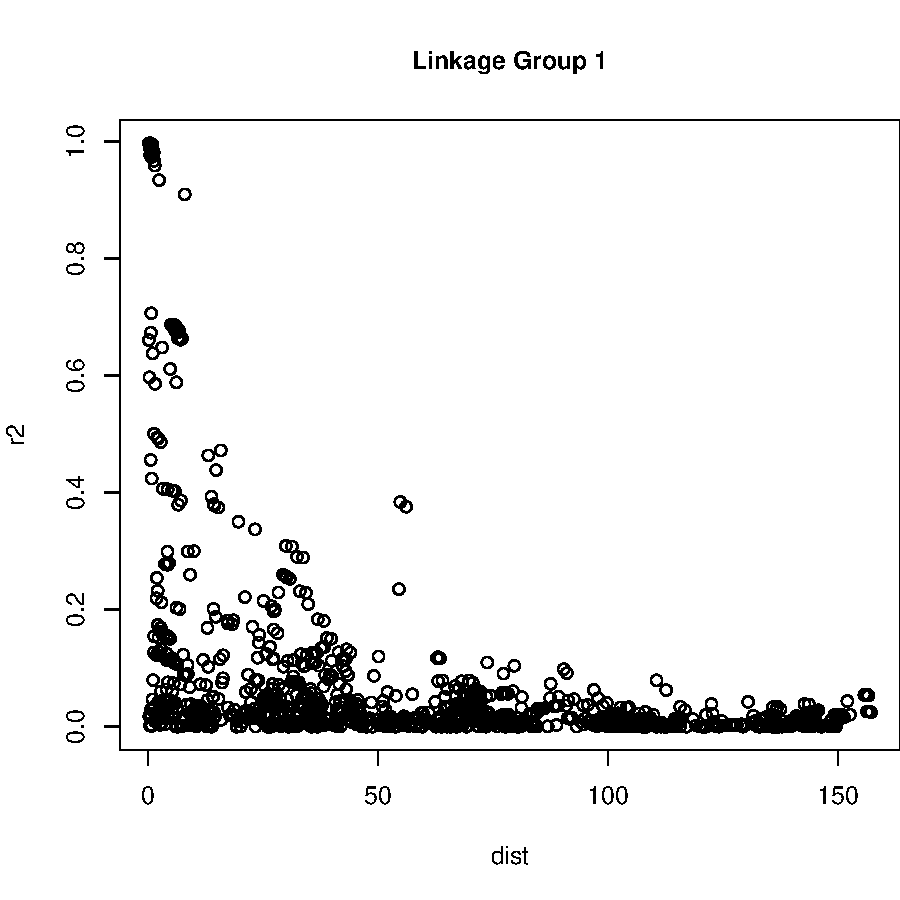
\includegraphics{figs/vignette-011}
\end{figure}    
      
It is possible to simulate a pedigree structure with function \texttt{simul.pedigree}. As arguments,
the number of generations to simulate and the number of individuals in each generation has to be specified. By default, random mating 
is assumed in each generation. As their are no further restrictions, it is possible that inbreeds could be generated when parent 1 equals parent 2.
To simulate a pedigree with 6 generations and 4, 6, 7, 9, 10 and 10 individuals in each generation, use
\begin{Schunk}
\begin{Sinput}
> set.seed(123)
> ped.simul <- simul.pedigree(gener = 6, ids = c(4, 6, 
+     7, 9, 10, 10))
\end{Sinput}
\end{Schunk}
The resulting pedigree is visualized in Figure \ref{fig:simupedi}.
\begin{figure}[!h]
\begin{Schunk}
\begin{Sinput}
> plot(ped.simul)
\end{Sinput}
\end{Schunk}
\includegraphics{figs/vignette-013}
\caption{Simulated pedigree structure}
\label{fig:simupedi}
\end{figure}

  

\section{Relationship matrices}\label{sec:RelationshipMatrices}  

Pedigree information is usually used to set up relationship matrices for a set of individuals. The relationship is constructed by the \textit{expected} fraction of alleles that are identical by descent (IBD) between relatives. Another possibility to set up a relationship is the use of marker data to compute the genomic relationship. This gives the \textit{observed} relationship of individuals.

\subsection{Based on Pedigree}

The computation of the pedigree based relationship in \texttt{synbreed} starts with the gametic relationship. A gamet is the genetic unit that an individual passes to its offspring. The genetic value of an individual at one locus consists of two allelels. 
Suppose there is an individual C with the parents A and B. Individual C has to alleles C1 and C2. The source of allele C1 is Parent A, thus allele C1 could either be IBD to A1 or A2. Allele C2 was inherited of parent B, thus it could be IBD to B1 or B2. 
To compute the gametic relationship start with an expanded table with two alleles for each individual. 
 
\begin{table}[!h]
\centering
\begin{tabular}{cccc}
\hline
ID & Allele & Par1 & Par2 \\
\hline
A & A1 & - & - \\
A & A2 & - & - \\
B & B1 & - & - \\
B & B1 & - & - \\
C & C1 & A1 & A2 \\
C & C2 & B1 & B2 \\
D & D1 & A1 & A2 \\
D & D2 & C1 & C2 \\
E & E1 & D1 & D2 \\
E & E2 & B1 & B2 \\
\hline
\end{tabular}
\end{table}

This table is converted into the gametic relationship $\bf G$ matrix which is of order $2n$, if the number of individuals is $n$. The diagonal values of $\bf G$ are always 1. The off-diagonal values give the probabilty that the two allelse are identical by
descent (IBD). If the parents are unknown, it is assumed that they are progeny of a random mating population. In this case the off-diagonals are zero. The other values of the gametic relations are filled in rowwise. 
The combination of $2^2=4$ alleles which describe the relationship of progeny A with parent C are computed as follows
$$ (A1,C1) = 0.5 \cdot [(A1,A1) + (A1,A2)] $$
$$ (A1,C2) = 0.5 \cdot [(A1,B1) + (A1,B2)] $$
$$ (A2,C1) = 0.5 \cdot [(A2,A1) + (A2,A2)] $$
$$ (A2,C2) = 0.5 \cdot [(A2,B1) + (A2,B2)] $$
The gametic relationship for a given pedigree is obtained as follows
\begin{Schunk}
\begin{Sinput}
> G <- kinship(ped, ret = "gam")
> G
\end{Sinput}
\begin{Soutput}
      A_1   A_2   B_1   B_2 C_1  C_2   D_1   D_2   E_1   E_2
A_1 1.000 0.000 0.000 0.000 0.5 0.00 0.500 0.250 0.375 0.000
A_2 0.000 1.000 0.000 0.000 0.5 0.00 0.500 0.250 0.375 0.000
B_1 0.000 0.000 1.000 0.000 0.0 0.50 0.000 0.250 0.125 0.500
B_2 0.000 0.000 0.000 1.000 0.0 0.50 0.000 0.250 0.125 0.500
C_1 0.500 0.500 0.000 0.000 1.0 0.00 0.500 0.500 0.500 0.000
C_2 0.000 0.000 0.500 0.500 0.0 1.00 0.000 0.500 0.250 0.500
D_1 0.500 0.500 0.000 0.000 0.5 0.00 1.000 0.250 0.625 0.000
D_2 0.250 0.250 0.250 0.250 0.5 0.50 0.250 1.000 0.625 0.250
E_1 0.375 0.375 0.125 0.125 0.5 0.25 0.625 0.625 1.000 0.125
E_2 0.000 0.000 0.500 0.500 0.0 0.50 0.000 0.250 0.125 1.000
attr(,"class")
[1] "relationshipMatrix"
\end{Soutput}
\end{Schunk}
The resulting object \texttt{G} is of class "relationshipMatrix" which is the general class for all kinds of relationship matrices (gametic relationship, additive and dominance relationship, kinship). An object of class "relationshipMatrix" is basically a symmetric matrix containing the relationship coefficient of two individuals.
Note that the entry of allele 1 and allele 2 of an individual $i$ equals his inbreeding coefficient $F_i$. For example, the inbreeding coefficent of individual D is
\begin{Schunk}
\begin{Sinput}
> G["D_1", "D_2"]
\end{Sinput}
\begin{Soutput}
[1] 0.25
attr(,"class")
[1] "relationshipMatrix"
\end{Soutput}
\end{Schunk}
which is nonzero because individuals A and C, which are the parents of D, are relatives. Once the gametic relationship is computed, it could be converted in the additive numerator relationship matrix $\bf A$ or the dominance relationship matrix $\bf D$. The additive relationship between the individuals A and B is given by
$$ 0.5 \cdot (G[A1,B1]+ G[A1,B2] + G[A2,B1] + G[A2,B2]),$$
where $G[.,.]$ denotes the corresponding value of the gametic relationship matrix $\bf G$. 

The additive numerator relationship matrix descripes the additive relationship between individuals and is of order $n$. 
It is typically used in the animal model to estimate breeding values (additive genetic effects)
\begin{equation}\label{eq:animalmodel}
 y_i = \mu + a_i + e_i,
\end{equation}                                        
where $y_i$ is the phenotypic value for individual $i$, $\mu$ the mean and $a_i$ is the additive genetic effect and $\bf a = (a_1,...,a_n)' \sim \text{N}(0,\bf{A} \sigma^2_a)$ is assumed.  For the residual,
$\bf e \sim \text{N}(0,\bf I \sigma^2)$ is assumeed. The additive numerator relationship matrix for a given pedigree is obtained as follows
\begin{Schunk}
\begin{Sinput}
> A <- kinship(ped, ret = "add")
> A
\end{Sinput}
\begin{Soutput}
      A     B     C    D     E
A 1.000 0.000 0.500 0.75 0.375
B 0.000 1.000 0.500 0.25 0.625
C 0.500 0.500 1.000 0.75 0.625
D 0.750 0.250 0.750 1.25 0.750
E 0.375 0.625 0.625 0.75 1.125
attr(,"class")
[1] "relationshipMatrix"
\end{Soutput}
\end{Schunk}
Note that the diagonals of $\bf A$ are $1+F_i$. Sometimes the kinship matrix is required, which is half of the additive numerator relationship matrix. It is obtained by
\begin{Schunk}
\begin{Sinput}
> K <- kinship(ped, ret = "kin")
\end{Sinput}
\end{Schunk}

Additionally it is possible to derive the dominance relationship matrix $\bf D$ out of $\bf G$. The dominance is needed in the non-additive animal model
\begin{equation}\label{eq:nonaddmodel}
y = \mu + a_i + d_{i} + e_i,
\end{equation}
with the same notation as in \eqref{eq:animalmodel} and $d_i$ being the dominance effect of individual $i$ with $\bf d  = (d_1,...,d_n) \sim  \text{N}(0,\bf{D} \sigma_d^2)$. The dominance relationship matrix
for the example pedigree is obtained  by
\begin{Schunk}
\begin{Sinput}
> D <- kinship(ped, ret = "dom")
> D
\end{Sinput}
\begin{Soutput}
     A     B    C       D        E
A 1.00 0.000 0.00 0.25000 0.000000
B 0.00 1.000 0.00 0.00000 0.125000
C 0.00 0.000 1.00 0.25000 0.250000
D 0.25 0.000 0.25 1.06250 0.156250
E 0.00 0.125 0.25 0.15625 1.015625
attr(,"class")
[1] "relationshipMatrix"
\end{Soutput}
\end{Schunk}
Variance-covariance matrices for effects of heigher order interactions in the non-additive animal model as addidive-additive (AA), additive-dominance (AD) or dominance-dominance (DD) variance-covariance matrices can be computes as
\begin{Schunk}
\begin{Sinput}
> (AA <- A * A)
\end{Sinput}
\begin{Soutput}
         A        B        C      D        E
A 1.000000 0.000000 0.250000 0.5625 0.140625
B 0.000000 1.000000 0.250000 0.0625 0.390625
C 0.250000 0.250000 1.000000 0.5625 0.390625
D 0.562500 0.062500 0.562500 1.5625 0.562500
E 0.140625 0.390625 0.390625 0.5625 1.265625
attr(,"class")
[1] "relationshipMatrix"
\end{Soutput}
\begin{Sinput}
> (AD <- A * D)
\end{Sinput}
\begin{Soutput}
       A        B       C         D         E
A 1.0000 0.000000 0.00000 0.1875000 0.0000000
B 0.0000 1.000000 0.00000 0.0000000 0.0781250
C 0.0000 0.000000 1.00000 0.1875000 0.1562500
D 0.1875 0.000000 0.18750 1.3281250 0.1171875
E 0.0000 0.078125 0.15625 0.1171875 1.1425781
attr(,"class")
[1] "relationshipMatrix"
\end{Soutput}
\begin{Sinput}
> (DD <- D * D)
\end{Sinput}
\begin{Soutput}
       A        B      C          D          E
A 1.0000 0.000000 0.0000 0.06250000 0.00000000
B 0.0000 1.000000 0.0000 0.00000000 0.01562500
C 0.0000 0.000000 1.0000 0.06250000 0.06250000
D 0.0625 0.000000 0.0625 1.12890625 0.02441406
E 0.0000 0.015625 0.0625 0.02441406 1.03149414
attr(,"class")
[1] "relationshipMatrix"
\end{Soutput}
\end{Schunk}
Model \eqref{eq:nonaddmodel} can be extended by these effects, but the contribution of three-way or higher interactions is usually small.  


\subsection{Based on marker data}

                 

The relationship matrix based on marker data or genomic relationship matrix data represents the true relationship between relatives
more precise than the numerator relationship based on pedigree, as it takes into account that relationship may deviate from the expected average relationship due to
Mendelian sampling effect.  Two methods for the construction of a relationship matrix based on marker data are implemented in the \texttt{synbreed} package: genomic relationship according to vanRaden \citep{vanRaden2008} and according to Roger's distance  \citep{Rogers1972}. 

For vanRaden, the SNP genotypes are coded as the number of copies of one of the SNP alleles, i.e., 0, 1 or 2 (any linear transformations of these values are valid too). Thus the marker data could be the result of a call of \texttt{codeGeno} when imputing for the missing values was performed or the missing values were replaced with the value 1.
The genomic relationship matrix according to vanRaden is computed as
\begin{equation}
\frac{\bf{Z}\bf{Z}'}{2\sum_{i=1}^p p_i(1-p_i)},
\end{equation}
where $\bf{Z}=\bf{M}-\bf{P}$ and $\bf{M}$ is the marker matrix and $\bf{P}$ contains the allele frequencies multiplied by 2. $p_i$ is the allele frequency of marker $i$.  As an example we look at the marker data of 6 individuals genotyped with 8 SNP markers. Let
$$ \bf M = \begin{pmatrix}  2 & 0 & 0 & 2 & 2 & 0 & 0 & 0 \\ 
   2 & 0 & 2 & 2 & 2 & 0 & 2 & 2 \\ 
   2 & 0 & 2 & 2 & 0 & 0 & 2 & 0 \\ 
   0 & 0 & 2 & 2 & 0 & 0 & 2 & 0 \\ 
   0 & 0 & 2 & 0 & 0 & 0 & 2 & 0 \\ 
   2 & 2 & 2 & 2 & 0 & 0 & 0 & 2 \\  
   \end{pmatrix}, $$
then it holds that
$$ \bf P = \begin{pmatrix}  1.33 & 0.33 & 1.67 & 1.67  & 0.67 & 0 &  1.33&  0.67 \\ 
   1.33 & 0.33 & 1.67 & 1.67  & 0.67 & 0 &  1.33&  0.67 \\ 
   1.33 & 0.33 & 1.67 & 1.67  & 0.67 & 0 &  1.33&  0.67 \\  
   1.33 & 0.33 & 1.67 & 1.67  & 0.67 & 0 &  1.33&  0.67 \\ 
   1.33 & 0.33 & 1.67 & 1.67  & 0.67 & 0 &  1.33&  0.67 \\  
   1.33 & 0.33 & 1.67 & 1.67  & 0.67 & 0 &  1.33&  0.67 \\   
   \end{pmatrix} $$
 $$    \bf Z = \begin{pmatrix}   0.67 & -0.33 & -1.67 & 0.33 & 1.33 & 0.00 & -1.33 & -0.67 \\ 
  0.67 & -0.33 & 0.33 & 0.33 & 1.33 & 0.00 & 0.67 & 1.33 \\ 
   0.67 & -0.33 & 0.33 & 0.33 & -0.67 & 0.00 & 0.67 & -0.67 \\ 
  -1.33 & -0.33 & 0.33 & 0.33 & -0.67 & 0.00 & 0.67 & -0.67 \\ 
   -1.33 & -0.33 & 0.33 & -1.67 & -0.67 & 0.00 & 0.67 & -0.67 \\ 
   0.67 & 1.67 & 0.33 & 0.33 & -0.67 & 0.00 & -1.33 & 1.33 \\ 
   \end{pmatrix}
  $$  
  and 
  $$ \bf Z \bf Z ' = \begin{pmatrix}  
   7.44 & 0.11 & -1.22 & -2.56 & -3.22 & -0.56 \\ 
   0.11 & 4.78 & -0.56 & -1.89 & -2.56 & 0.11 \\ 
   -1.22 & -0.56 & 2.11 & 0.78 & 0.11 & -1.22 \\ 
   -2.56 & -1.89 & 0.78 & 3.44 & 2.78 & -2.56 \\ 
   -3.22 & -2.56 & 0.11 & 2.78 & 6.11 & -3.22 \\ 
   -0.56 & 0.11 & -1.22 & -2.56 & -3.22 & 7.44 \\
     \end{pmatrix}
  $$  
with the denominator being $2\sum_{i=1}^p p_i(1-p_i)=2.611$. To compute the genomic relationship according to vanRaden, matrix $\bf M$ is passed to the funtion \texttt{vanRaden}  
\begin{Schunk}
\begin{Sinput}
> M <- matrix(data = c(2, 0, 0, 2, 2, 0, 0, 0, 2, 0, 2, 
+     2, 2, 0, 2, 2, 2, 0, 2, 2, 0, 0, 2, 0, 0, 0, 2, 2, 
+     0, 0, 2, 0, 0, 0, 2, 0, 0, 0, 2, 0, 2, 2, 2, 2, 0, 
+     0, 0, 2), nrow = 6, byrow = TRUE)
> vR <- vanRaden(M)
> round(vR, 3)
\end{Sinput}
\begin{Soutput}
       [,1]   [,2]   [,3]   [,4]   [,5]   [,6]
[1,]  2.851  0.043 -0.468 -0.979 -1.234 -0.213
[2,]  0.043  1.830 -0.213 -0.723 -0.979  0.043
[3,] -0.468 -0.213  0.809  0.298  0.043 -0.468
[4,] -0.979 -0.723  0.298  1.319  1.064 -0.979
[5,] -1.234 -0.979  0.043  1.064  2.340 -1.234
[6,] -0.213  0.043 -0.468 -0.979 -1.234  2.851
attr(,"class")
[1] "relationshipMatrix"
\end{Soutput}
\end{Schunk}
Note the object \texttt{vR} is again of class "relationshipMatrix".    

Another possibility is to compute the genomic relationship matrix according to Roger's distance. Roger's distance is computed as 
\begin{equation}
d=\frac{1}{p}\sum_{i=1}^p \sqrt{1/2 \sum_{j=1}^{n_i}(p_{ij}-q_{ij})^2}
\end{equation}
where $p$ is the number of markers and $n_i$ is the number of alleles for marker $i$. Let $p_{ij}$ and $q_{ij}$ denote the allele frequencies of allele $j$ for marker $i$ respectively. Note that marker data should be coded $-1$ and $1$ for homozygous genotypes and 0 for heterozygous. If marker data is code 0/1/2 data is transformed automatically
when funtion \texttt{rogers} is used, which computes Roger's distance.  



\subsection{Doubled haploid lines}

In plant breeding doubled haploid (DH) lines are common. DH lines are fully inbreed and thus have an inbreeding coefficient of 1. This has to be taken into account, when the relationship matrix in a pedigree with DH lines is computed.  As an example the \texttt{maize} data is taken.
\begin{Schunk}
\begin{Sinput}
> data(maize)
> head(maize.ped)
\end{Sinput}
\begin{Soutput}
  ID Par1 Par2 DH
1  1    0    0  1
2  2    0    0  1
3  3    0    0  1
4  4    0    0  1
5  5    0    0  1
6  6    0    0  1
\end{Soutput}
\end{Schunk}
First, the additive numerator relationship matrix is computed. There are 1276 DH lines and 25 non DH lines in the pedigree. For DH lines special treatment is necassary, as the inbreeding coefficient must be 1. An argument \texttt{DH} is available for function \texttt{kinship} where
for each individual in the pedigree it specified whether this is a DH line or not. This information is available for the \texttt{maize} data. To obtain the addtive numerator relationship matrix of the first 100 genotypes, use 
\begin{Schunk}
\begin{Sinput}
> ped.maize <- create.pedigree(maize.ped$ID, maize.ped$Par1, 
+     maize.ped$Par2)
> A.maize100 <- kinship(ped.maize[1:100, ], DH = maize.ped$DH[1:100], 
+     ret = "add")
> dim(A.maize100)
\end{Sinput}
\begin{Soutput}
[1] 100 100
\end{Soutput}
\end{Schunk}

\subsection{Visualisation of relationship matrices}

As in most cases a relationship matrix is to big to print it on the screen. Thus there are two possibilites for visualisation of an object of class "relationshipMatrix" in \texttt{synbreed} package. A \texttt{summary} method is defined which gives the important characteristics of a relationship matrix. Use
\begin{Schunk}
\begin{Sinput}
> summary(A.maize100)
\end{Sinput}
\begin{Soutput}
Dimension         : 100 x 100 
Rank              : 75 
Range             : 0 -- 2 
# of unique values: 5 
\end{Soutput}
\end{Schunk}
to get the summary for the pedigree based additive relationship matrix of the \texttt{maize} data. Another possibility is the \texttt{plot} method which could be applied
to an object of class "relationshipMatrix". This gives a heatmap of the entries of the relationship matrix
%\begin{figure}
%<<fig=TRUE>>=
%plot(A.maize100)
%@
%\caption{Heatmap of pedigree based additive relationship matrix for \texttt{maize} data.}
%\label{fig:heatpedi}
%\end{figure}
%In Figure \ref{fig:heatpedi} one can see the family  structure in the data which is consiting of 25 families.

Note that objects of class "relationshipMatrix" can be writen two input files appropriate for Mixed Model software as \texttt{WOMBAT} \citep{Meyer2006} or \texttt{ASReml} \citep{Gilmour2000}.


\section{Acknowledgements}

This research was funded by the German Federal Ministry of Education and
Research (BMBF) within the AgroClustEr \textit{Synbreed} $-$  \textit{Synergistic plant and
animal breeding}.

  \bibliography{references}

\end{document}                                                                                                                                                       
